\documentclass[10pt,compress]{beamer}
%\documentclass[10pt,compress,draft]{beamer}
\mode<presentation>
\usepackage{graphicx}
%\usepackage{beamerthemesplit}
\usepackage[ansinew]{inputenc}
%\usepackage[spanish]{babel}
\usepackage{amsmath,amssymb}
\usepackage{eqlist}
\usepackage{amsfonts} % Simbolos matematicos
\usepackage{amsthm} %Enunciados predefinidos y demostraciones
\usepackage{bbm}
\usepackage{enumerate}
\usepackage[dvips]{epsfig} %Incluir figuras .eps
\usepackage{epsf}%Incluir figuras .eps
\usepackage{eurosym}
\usepackage{subfigure}
\usepackage{graphicx}
\useoutertheme[footline=authortitle]{miniframes}
\useinnertheme{circles}
\usepackage{multirow}
\usepackage{animate}
\usepackage{booktabs}
\usepackage{siunitx}

\usepackage{chicago}%,e:/latex/psfrag

%%%%%%%%%%
%    1   %
%%%%%%%%%%
\title[Multidimensional Scaling for Big Data\qquad{} MESIO  \qquad{} \insertframenumber %/54]
%/\inserttotalframenumber]
/\pageref{last_page}]
{\LARGE Multidimensional Scaling for Big Data}
\author[Cristian Pach\'on Garc\'ia]{{
   \large Cristian Pach\'on Garc\'ia \\
    \small Advisor: Pedro Delicado Useros
  }
\\
%{\small January 2019}
}
\date{\today}

\usepackage{Sweave}
\begin{document}
\Sconcordance{concordance:presentation.tex:presentation.Rnw:%
1 43 1 1 0 595 1}


\frame{\titlepage}


\frame{\scriptsize{\tableofcontents} }
\AtBeginSubsection[]
{
  \begin{frame}<beamer>
    \frametitle{}
    \scriptsize{\tableofcontents[currentsection,currentsubsection]}
  \end{frame}
}

\AtBeginSection[]
{
  \begin{frame}<beamer>
   \frametitle{}
    \scriptsize{\tableofcontents[currentsection,currentsubsection]}
  \end{frame}
}

%%%%%%%%%%%%%%%%%%%%%%%%%%%%%%%%%%%%%%%%%%%%%%%%%%%%%%%%
\section{Introduction}

%%%%%%%%%%%%%%%%%%%%%%%%
\frame{\frametitle{What is MDS?}
\begin{itemize}
\item MDS is a statistic tool for reduction of dimensionality, using as input 
a distance matrix.

\item Given a square matrix \textbf{D} $n\times n$, the goal of MDS is to 
obtain a configuration matrix \textbf{X} $n \times q$ satisfying:

\begin{itemize}
\item Columns are orthogonal. 

\item The Euclidean distance between the rows of \textbf{X} 
is approximately equal to \textbf{D}. 


\end{itemize}

\item \textbf{X} can be interpreted as the matrix of $q$ \textbf{latent}
variables for the $n$ observations.

\item The columns of \textbf{X} are called \textit{principal coordinates}.


\end{itemize}
}



%%%%%%%%%%%%%%%%%%%%%%%%
\frame{\frametitle{Example}
Consider the distance between some cities of Europe, as shown in the following 
matrix:

\begin{table}[ht]
\centering
\begin{tabular}{rrrrrrr}
 & Athens & Barcelona & Brussels & Calais & Cherbourg & $\dotsi$ \\ 
  \hline
Athens & 0 & 3313 & 2963 & 3175 & 3339 & $\dotsi$ \\ 
  Barcelona & 3313 & 0& 1318 & 1326 & 1294 & $\dotsi$ \\ 
  Brussels & 2963 & 1318 & 0 & 204 & 583 & $\dotsi$ \\ 
  Calais & 3175 & 1326 & 204 & 0 & 460 & $\dotsi$ \\ 
  Cherbourg & 3339 & 1294 & 583 & 460 & 0 & $\dotsi$ \\
  $\vdots$ & $\vdots$ & $\vdots$ & $\vdots$ & $\vdots$ & $\vdots$ & $\ddots$ \\
   \hline
\end{tabular}
\caption{Distances between European cities (just 5 of them are shown).} 
\label{european_distances}
\end{table}

}

\frame{
\begin{figure}
    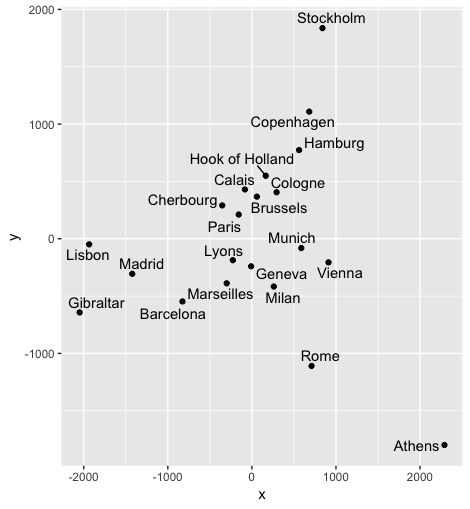
\includegraphics[width=\textwidth,height=0.8\textheight,keepaspectratio]{./images/europ_cities.png}
    \caption{MDS configuration for European cities}
\end{figure}
}


\frame{
\begin{figure}
    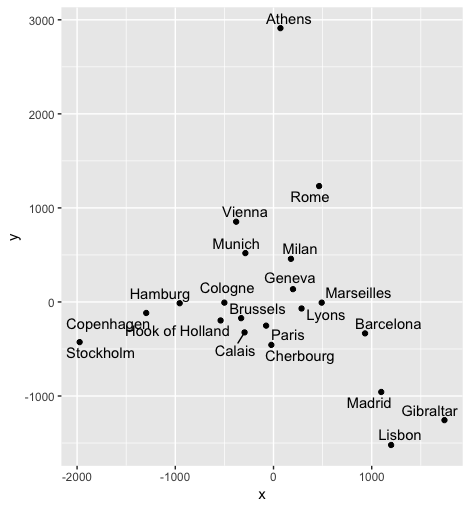
\includegraphics[width=\textwidth,height=0.8\textheight,keepaspectratio]{./images/europ_cities_rot.png}
    \caption{(Another) MDS configuration for European cities}
\end{figure}

}

\frame{\frametitle{Procrustes transformation} 
\begin{itemize}

\item Given a MDS configuration, any rotation, reflection or translation is a 
valid MDS configuration, since they preserve the distance. So, the solution 
is not unique.

\item Procrustes transformation problem:
\begin{itemize}
\item Let \textbf{A} and \textbf{B} be two different MDS configurations 
for the same set of data. One wants to obtain 
$s$, $\mathbf{T}$ and $\mathbf{t}$ such that

\[
\mathbf{A} = s \mathbf{B} \mathbf{T} + \mathbf{1t}',
\]
where \textbf{T} is an orthogonal matrix. 

\item In \citeN{BorgGroenen2005} are all the details needed to estimate 
these parameters.

\end{itemize}
\end{itemize}
}




%%%%%%%%%%%%%%%%%%%%%%%%%%%%%%%%%%%%%%%%%%%%%%%%%%%%%%%%
\section{Algorithms for MDS with Big Data}

\frame{\frametitle{Why is it needed?}

\begin{figure}
    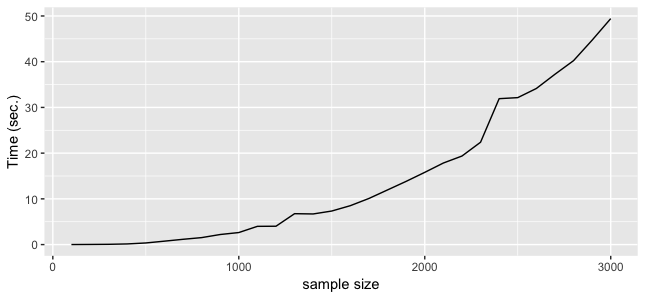
\includegraphics{./images/elapsed_time_mds.png}
    \caption{Elapsed time to compute MDS.}
\end{figure}

}

\frame{

\begin{figure}
    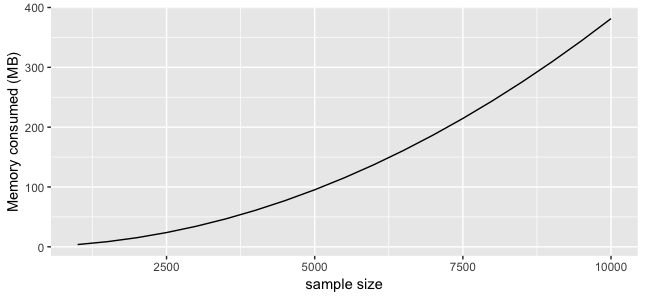
\includegraphics{./images/memory_distance.png}
    \caption{Memory consumed to compute the distance matrix.}
\end{figure}

}


%%%%%%%%%%%%%%%%%%%%%%%%
\frame{\frametitle{Three algorithms for MDS with Big Data}
\begin{itemize}

\item \textit{Divide and Conquer MDS:}
\begin{itemize}
\item First approach of this thesis.
\end{itemize}

\item \textit{Fast MDS:}
\begin{itemize}
\item It uses recursive programming.
\item Developed by \citeN{Yang06afast}.
\end{itemize}

\item \textit{MDS based on Gower interpolation:}
\begin{itemize}
\item It adds a new set of points to an existing MDS configuration.
\item See Appendix of \cite{gowerformula}.
\end{itemize}

\end{itemize}
}





%%%%%%%%%%%%%%%%%%%%%%%%
\frame{\frametitle{Divide and Conquer MDS}
  \centering
  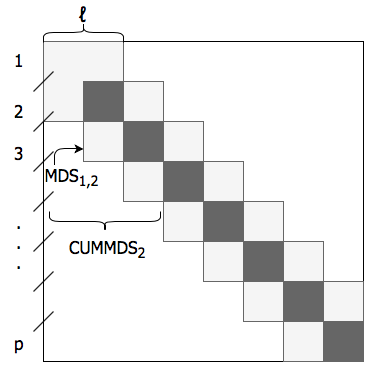
\includegraphics[width=\textwidth,height=0.8\textheight,keepaspectratio]{./images/div_conq_alg.png}
  
}

%[width=\textwidth,height=0.8\textheight,keepaspectratio]
\frame{\frametitle{Fast MDS}
\begin{figure}
    \centering
    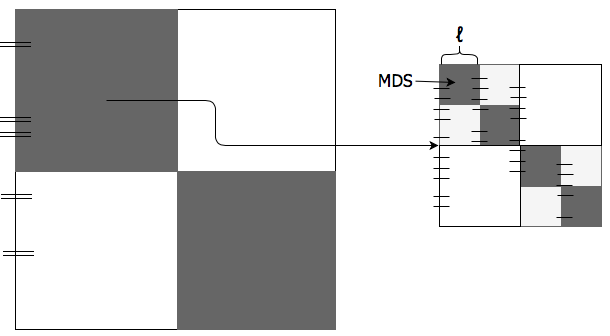
\includegraphics{./images/fast_mds_alg.png}
\end{figure}
}


\frame{\frametitle{MDS based on Gower interpolation}
\begin{figure}
    \centering
    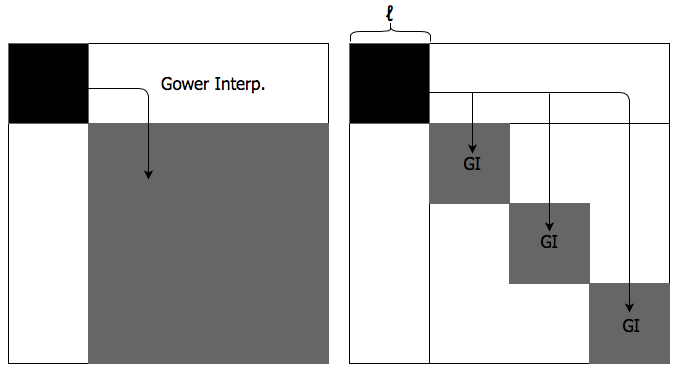
\includegraphics{./images/gi_alg.png}
\end{figure}
}


%%%%%%%%%%%%%%%%%%%%%%%%
\frame{\frametitle{Output of the algorithms}
The three algorithms have the same type of output. It consists on a list of 
two parameters, which are

\begin{itemize}
\item A MDS configuration for the initial dataset.

\item The second parameter is a list of eigenvalues.

\end{itemize}

}



%%%%%%%%%%%%%%%%%%%%%%%%%%%%%%%%%%%%%%%%%%%%%%%%%%%%%%%%
\section{Simulation study}
\frame{\frametitle{Simulation study}


Given the three algorithms, we would like to explore their performance:

\begin{itemize}
\item Performance in terms of results quality: are they able to capture 
the right data dimensionality?

\item Performance in terms of time: are they `` fast" 
enough? Which one is the fastest?

\end{itemize}

}

%%%%%%%%%%%%%%%%%%%%%%%%
\subsection{Design of the simulation}
\frame{\frametitle{Design of the simulation}

\begin{itemize}
\item \textit{Sample sizes}: A total of six sample sizes are used, which are:

\begin{itemize}
\item Small sample sizes: $10^3, 3\cdot 10^3, 5\cdot 10^3$ and $10^4$.

\item Large sample sizes: $10^5$ and $10^6$.

\end{itemize}

\item \textit{Data dimensions}: we generate a matrix with two different number 
of columns: 10 and 100.

\item \textit{Main dimensions}: Postmultiplication by a diagonal matrix:

\begin{itemize}
\item Identity matrix (\textit{noisy scenarios}).

\item One main dimension with $\lambda$: 15.

\item  Two main dimensions of the same value $\lambda$: 15.

\item  Two main dimensions of different values $\lambda$: 15, 10.

\item  Four main dimensions of the same value $\lambda$: 15.
\end{itemize}

\item As a probabilistic model, we use a Normal distribution.

\item Given a scenario, it is replicated 100 times.

\end{itemize}
}


\frame{
\begin{enumerate}

\item Generate the dataset \textbf{X} according to the scenario. 

\item For each algorithm, we do the following steps:

\begin{enumerate}

\item Run the algorithm and get MDS configuration for the algorithm
($\mathbf{MDS_{alg}}$).

\item Get the elapsed time to compute MDS configuration and store it.

\item Get eigenvalues and store them.

\item Align $\mathbf{MDS_{alg}}$ and \textbf{X} using (Partition) Procrustes.

\item Get the correlation coefficients between the main dimensions of 
$\mathbf{MDS_{alg}}$ and \textbf{X} and store them.

\end{enumerate}
\end{enumerate}
}


\frame{

\begin{itemize}
\item Performance of results quality:
\begin{itemize}


\item Correlation between the main dimensions of the data and the
main dimensions after applying the algorithms. We get the diagonal of the 
correlation matrix. 

\item \textit{Eigenvalues} as an approximation of the standard 
deviation of the variables of \textbf{X}.
\end{itemize}

\item Elapsed Time to get the MDS configuration.

\end{itemize}

}

%%%%%%%%%%%%%%%%%%%%%%%%
\subsection{Results}
\frame{\frametitle{Correlation coefficients}
\begin{figure}
%\begin{minipage}{\textwidth}
    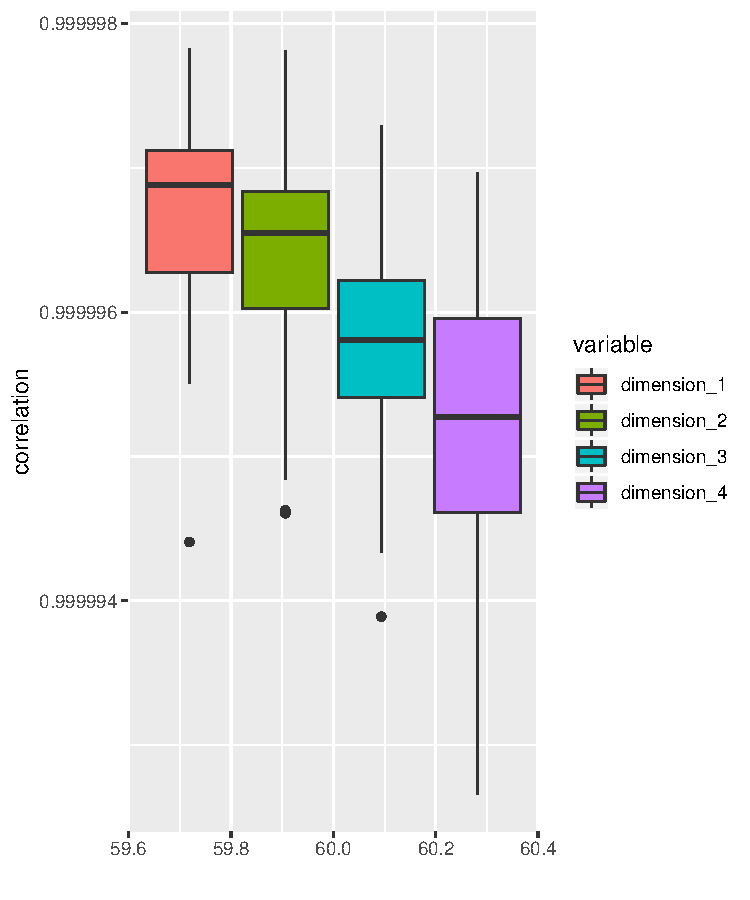
\includegraphics[width=\textwidth,height=0.7\textheight,keepaspectratio]{./images/example_corr_divide.pdf}
    \caption{
    Correlation coefficients between the main dimensions of \textbf{X} 
    and the main dimensions of $\mathbf{MDS_{Div}}$ for
    a scenario with $n=10^6$, 100 columns and 
    4 main dimensions with $\lambda = 15$.}
%\end{minipage}
\end{figure}
}

\frame{

\begin{figure}
%\begin{minipage}{\textwidth}
    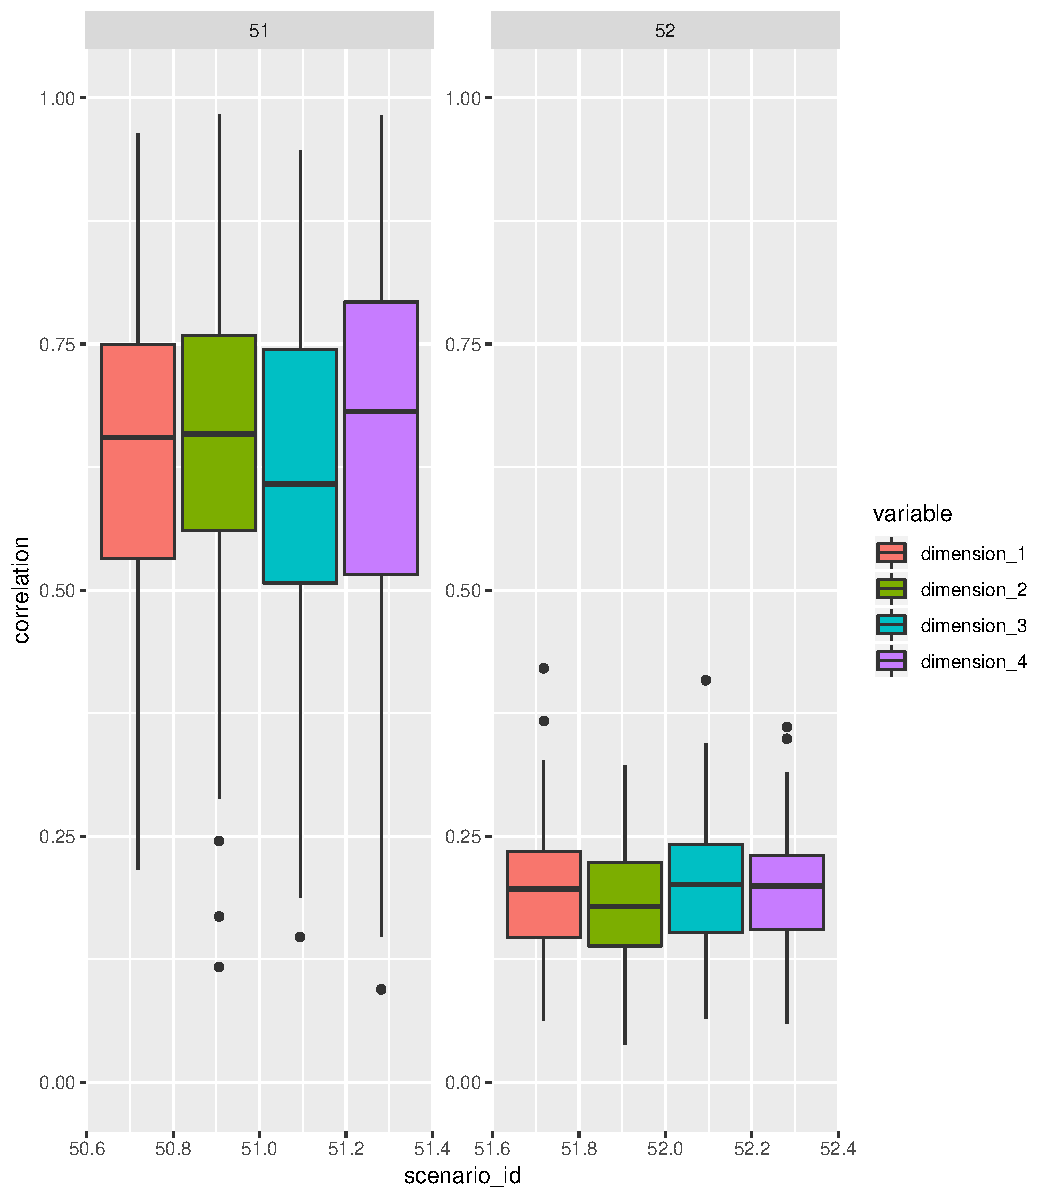
\includegraphics[width=\textwidth,height=0.7\textheight,keepaspectratio]{./images/noisy_corr_divide.pdf}
    \caption{
    Correlation coefficients between \textbf{X} and 
    $\mathbf{MDS_{Div}}$ for two different \textit{noise scenarios} 
    } 
%\end{minipage}
\end{figure}
}



%%%%%%%%%%%%%%%%%%%%%%%%
\frame{\frametitle{Eigenvalues}
\begin{itemize}
\item Since the original dataset, \textbf{X}, is postmultiplied by a diagonal 
matrix $k \times k$ that contains $\lambda_1, \dots, \lambda_k$, then 
$\mbox{var}(X_i) = \lambda_i^2$ and $\mbox{sd}(X_i) = \lambda_i$.


\item Let $\phi_1, \dots, \phi_t$ be the 
\textit{eigenvalues} of the MDS configuration such that 
$\phi_1 > \phi_2 > \cdots > \phi_t$. The first highest
\textit{eigenvalues} have to verify $\sqrt{\phi_j} \approx \lambda_j$.

\item We compute the bias.

\end{itemize}


}


\frame{
\begin{table}
  \begin{tabular}{rr|rr|rr|rr}
    \hline
     \multicolumn{2}{r|}{} & 
      \multicolumn{2}{c|}{Div. Conq. MDS} & 
       \multicolumn{2}{c|}{Fast} &
       \multicolumn{2}{c}{Gower MDS}\\
      sample\_size & n\_dim & $\overline{\sqrt{\phi}}$ & $\widehat{\mbox{bias}}$  & $\overline{\sqrt{\phi}}$ & $\widehat{\mbox{bias}}$ & $\overline{\sqrt{\phi}}$ & $\widehat{\mbox{bias}}$\\
      \hline
      $10^3$ & 10  & 14.98 & -0.02 & 15.85 & 0.15 & 15.05 & 0.05  \\ 
      $10^3$ & 100  & 15.03 & 0.03 & 15.01 & 0.01 & 15.02 & 0.02  \\ 
      $3 \cdot 10^3$ & 10  & 15.00 & -0.00 & 14.91 & -0.09 & 14.04 & -0.06  \\ 
      $3 \cdot 10^3$ & 100  & 14.96 & -0.04 & 15.10 & 0.10 & 15.04 & 0.04  \\ 
      $5 \cdot 10^3$ & 10 &  14.99 &  -0.01 & 14.96 & -0.04 & 14.98 & -0.02  \\ 
      $5 \cdot 10^3$ & 100 &  14.99 & -0.01 & 15.03 & 0.03 &15.02 & 0.02  \\ 
      $10^4$ & 10  & 14.99 & -0.01 & 14.33 & -0.67  & 14.99 & -0.01\\ 
      $10^4$ & 100  & 14.99 & -0.01 & 15.09 & 0.09 & 15.06 & 0.06\\ 
      $10^5$ & 10  & 14.99 & -0.01 & 15.00 & 0.00 & 15.04 & 0.04  \\ 
      $10^5$ & 100  & 14.99 & -0.01 & 15.00 &0.00 & 14.97 & -0.03  \\ 
      $10^6$ & 10  & 14.98 & -0.02 & 14.86 & -0.14 & 14.98 & -0.02  \\ 
      $10^6$ & 100  & 14.99 & -0.01 & 14.90 & -0.10 & 14.90 & -0.10 \\ 
    \bottomrule
  \end{tabular}
  \caption{Estimator and $\widehat{\mbox{bias}}$ for 
       scenarios with one main dimension $\lambda = 15$.}
\end{table}

}


%\frame{
%\begin{table}[ht]
%\centering
%\begin{tabular}{rrrr}
% scenario\_id & $\overline{\sqrt{\phi_1}}$ & $\widehat{\mbox{bias}_1}$ & $\widehat{\mbox{MSE}_1}$ \\
%  \hline
%  3 & 14.85 & -0.15 & 2.27 \\ 
%  4 & 15.01 & 0.01 & 0.01 \\ 
%  13 & 14.91 & -0.09 & 0.76 \\ 
%  14 & 15.10 & 0.10 & 0.93 \\ 
%  23 & 14.96 & -0.04 & 0.14 \\ 
%  24 & 15.03 & 0.03 & 0.07 \\ 
%  33 & 14.33 & -0.67 & 44.82 \\ 
%  34 & 15.09 & 0.09 & 0.76 \\ 
%  43 & 15.00 & -0.00 & 0.00 \\ 
%  44 & 15.00 & 0.00 & 0.00 \\ 
%  53 & 14.86 & -0.14 & 1.88 \\ 
%  54 & 14.90 & -0.10 & 1.02 \\ 
%   \hline
%\end{tabular}
%\caption{Estimator, $\widehat{\mbox{bias}}$ and $\widehat{\mbox{MSE}}$ for scenarios with one main dimension %$\lambda_1 = 15$ for \textit{Fast MDS}.}
%\label{mse_fast_one_dimensions}
%\end{table}
%
%}
%
%\frame{
%\begin{table}[ht]
%\centering
%\begin{tabular}{rrrr}
% scenario\_id & $\overline{\sqrt{\phi_1}}$ & $\widehat{\mbox{bias}_1}$ & $\widehat{\mbox{MSE}_1}$\\
%  \hline
%  3 & 15.05 & 0.05 & 0.22 \\ 
%  4 & 15.02 & 0.02 & 0.04 \\ 
%  13 & 14.94 & -0.06 & 0.36 \\ 
%  14 & 15.04 & 0.04 & 0.20 \\ 
%  23 & 14.98 & -0.02 & 0.04 \\ 
%  24 & 15.02 & 0.02 & 0.05 \\ 
%  33 & 14.99 & -0.01 & 0.01 \\ 
%  34 & 15.06 & 0.06 & 0.31 \\ 
%  43 & 15.04 & 0.04 & 0.19 \\ 
%  44 & 14.97 & -0.03 & 0.07 \\ 
%  53 & 14.98 & -0.02 & 0.06 \\ 
%  54 & 14.90 & -0.10 & 1.07 \\ 
%   \hline
%\end{tabular}
%\caption{Estimator, $\widehat{\mbox{bias}}$ and $\widehat{\mbox{MSE}}$ for scenarios with one main dimension %$\lambda_1 = 15$ for \textit{MDS based on Gower interpolation}.}
%\label{mse_gower_one_dimensions}
%\end{table}
%}



%%%%%%%%%%%%%%%%%%%%%%%%
\frame{\frametitle{Time to compute MDS}
\begin{table}[ht]
\centering
\begin{tabular}{rrrrr}
 sample\_size & n\_dim & mean\_divide\_conquer & mean\_fast & mean\_gower \\ 
  \hline
  $10^3$ & 10 & 0.27 & 0.14 & 0.10 \\ 
  $10^3$ & 100 & 0.78 & 0.69 & 0.28 \\ 
  $3 \cdot 10^3$ & 10 & 0.78 & 0.32 & 0.16 \\ 
  $3 \cdot 10^3$ & 100 & 2.50 & 3.14 & 0.52 \\ 
  $5 \cdot 10^3$ & 10 & 1.37 & 0.54 & 0.20 \\ 
  $5 \cdot 10^3$ & 100 & 4.25 & 5.69 & 0.84 \\ 
  $10^4$ & 10 & 2.60 & 1.81 & 0.31 \\ 
  $10^4$ & 100 & 8.85 & 11.79 & 1.37 \\ 
  $10^5$ & 10 & 28.10 & 11.46 & 2.44 \\ 
  $10^5$ & 100 & 106.30 & 116.46 & 18.02 \\ 
  $10^6$ & 10 & 420.29 & 106.59 & 53.15 \\ 
  $10^6$ & 100 & 2365.46 & 1070.19 & 813.15 \\ 
   \hline
\end{tabular}
\caption{Mean of elapsed time (in seconds) to compute each algorithm.} 
\label{mean_elapsed_time}
\end{table}
}


\frame{
\begin{itemize}
\item We do an \textsf{ANOVA} test using three factors: 

\begin{itemize}
\item The sample size, which has 6 levels.
\item The number of dimensions, which has 2 levels.
\item The algorithm, which has 3 levels.
\end{itemize}
\item Instead of using the \textit{elapsed time} variable, we use its logarithm.
\end{itemize}

}


\frame{
\begin{table}[ht]
\centering
\begin{tabular}{rrrrr}
 & Estimate & Std. Error & t value & Pr($>$$|$t$|$) \\ 
  \hline
(Intercept) & -1.4058 & 0.0085 & -165.44 & $<2e-16$ \\ 
  algorithmfast & -0.4313 & 0.0069 & -62.17 & $<2e-16$ \\ 
  algorithmgower & -1.6926 & 0.0069 & -243.96 & $<2e-16$ \\ 
  sample\_size3000 & 0.9473 & 0.0098 & 96.54 & $<2e-16$ \\ 
  sample\_size5000 & 1.4434 & 0.0098 & 147.10 & $<2e-16$ \\ 
  sample\_size10000 & 2.1505 & 0.0098 & 219.17 & $<2e-16$ \\ 
  sample\_size1e+05 & 4.4286 & 0.0098 & 451.35 & $<2e-16$ \\ 
  sample\_size1e+06 & 7.2782 & 0.0098 & 741.78 & $<2e-16$ \\ 
  n\_dimensions100 & 1.6910 & 0.0057 & 298.51 & $<2e-16$ \\ 
   \hline
\end{tabular}
\caption{Linear model for response $\log(\mbox{elapsed\_time})$.} 
\label{lm_all_variables}
\end{table}
}


\frame{

\begin{figure}
\centering
%\begin{minipage}{\textwidth}
    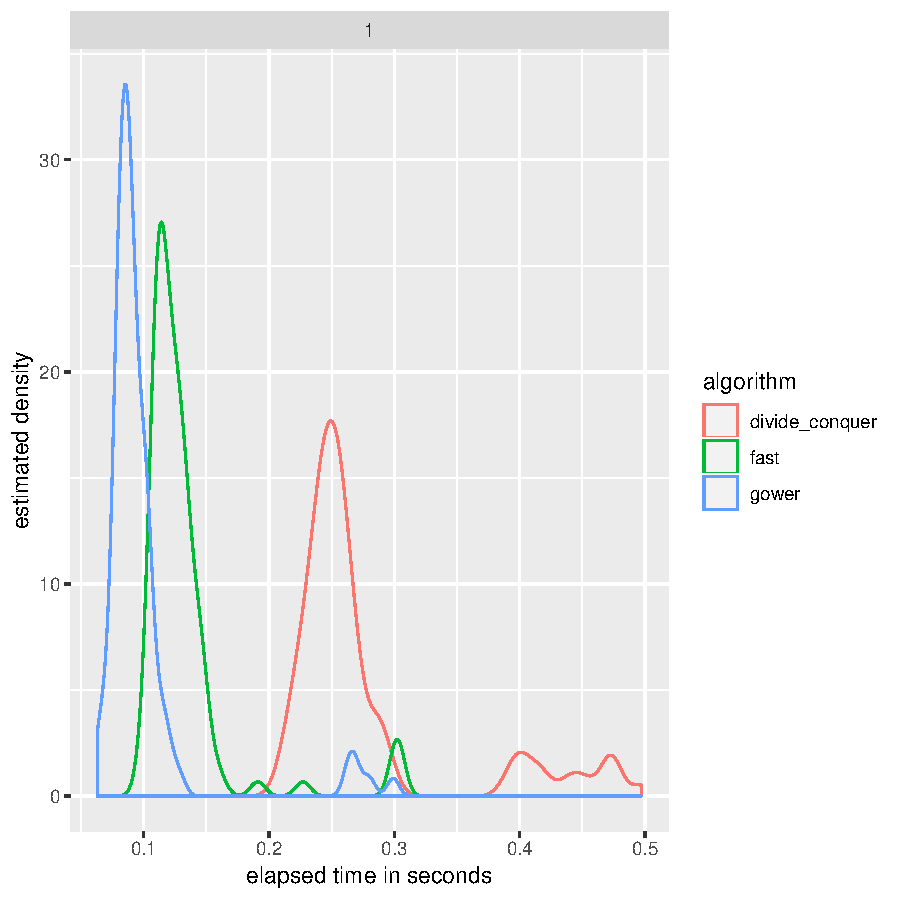
\includegraphics[width=\textwidth,height=0.8\textheight,keepaspectratio]{./images/scenario_id_1.pdf}
    \caption{
    Estimated density of elapsed time (in sec.) for each algorithm and 
    scenario with $n=10^3$, 10 columns and $\lambda_i = 1$ $i \in \{1,\dots,10\}$.
    }
%\end{minipage}
\end{figure}

}

\frame{

\begin{figure}
\centering
%\begin{minipage}{\textwidth}
    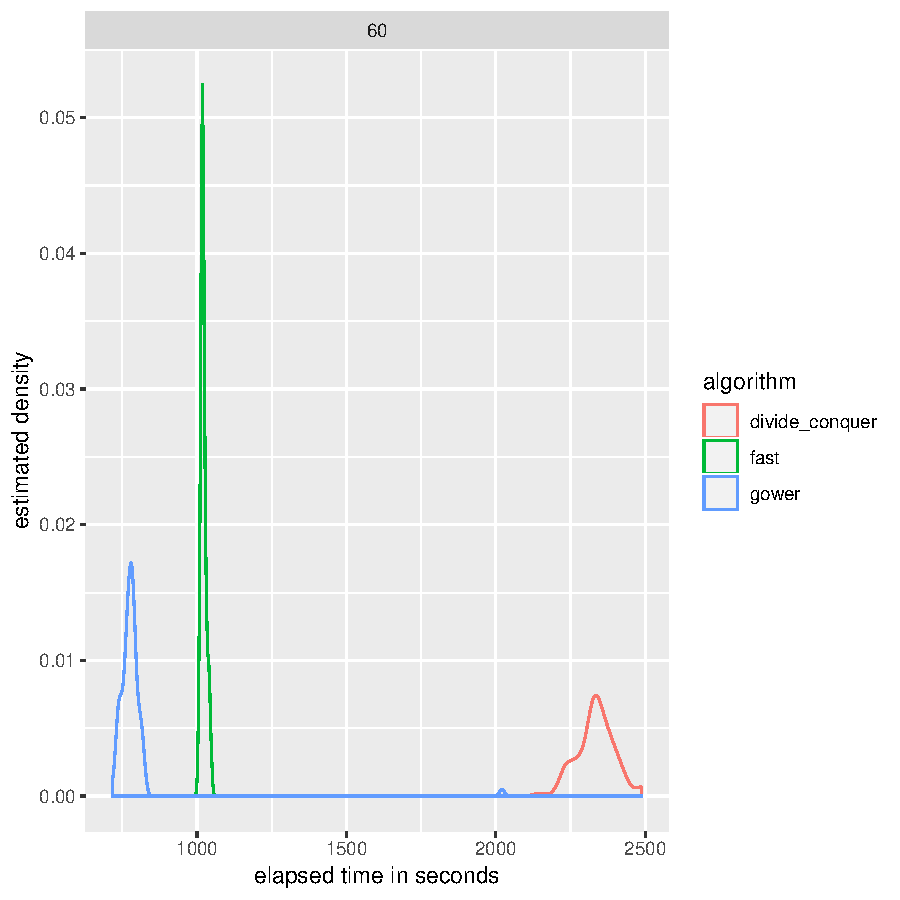
\includegraphics[width=\textwidth,height=0.8\textheight,keepaspectratio]{./images/scenario_id_60.pdf}
    \caption{
    Estimated density of elapsed time (in sec.) for each algorithm and 
    scenario with $n=10^6$, 100 columns and 4 main dimensions with 
    $\lambda = 15$.
    }
%\end{minipage}
\end{figure}

}

%%%%%%%%%%%%%%%%%%%%%%%%%%%%%%%%%%%%%%%%%%%%%%%%%%%%%%%%
\section{Conclusions}
\frame{\frametitle{Conclusions}
\begin{itemize}

\item The fastest algorithm is \textit{MDS based on Gower interpolation}. 
\item \textit{Fast MDS} is able to obtain a MDS configuration in a reasonable
amount of time. 
\item The best algorithm capturing the variance of the original dataset is
\textit{Divide and Conquer MDS}.
\item \textit{MDS based on Gower interpolation} is the best choice,
since it is the fastest algorithm and its results quality are good. 
\item This algorithm does essentially what classical Statistics advises: 
when your population is too large, take a sample of it.
\end{itemize}
}


\frame{\frametitle{Next steps}
\begin{itemize}

\item Modify \textit{Divide and Conquer} in order to use less points for 
Procrustes. 
\item Use \textit{real datasets} with the algorithms. 
\item Build and \textsf{R} library.

\end{itemize}
}

%%%%%%%%%%%%%%%%%%%%%%%%%%%%%%%%%%%%%%%%%%%%%%%%%%%%%%%%
\begin{frame}
  \centering \Huge
  \emph{Thank You}
\end{frame}

%%%%%%%%%%%%%%%%%%%%%%%%%%%%%%%%%%%%%%%%%%%%%%%%%%%%%%%%
\bibliographystyle{chicago}
{


\bibliography{bibliography.bib} %,DataMining}
\label{last_page}
}




\end{document}
